% !TeX program = xelatex
\documentclass[12pt]{article}
\usepackage[right=1.0in,left=1.0in,top=1.0in,bottom=1.0in]{geometry}
\usepackage{hyperref}
\hypersetup{colorlinks, citecolor=blue, filecolor=blue, linkcolor=blue, urlcolor=blue}
\usepackage{graphicx}
\usepackage{url}
\usepackage[round]{natbib}
\usepackage{amsmath,amsthm,amssymb}
\usepackage{booktabs}
\usepackage{multirow}
\usepackage{float}
\usepackage{pdflscape}
\usepackage[labelsep=period]{caption}
\usepackage{subcaption}
\usepackage{longtable}
\usepackage{threeparttable}
\usepackage{threeparttablex}
\usepackage{environ}

\usepackage{setspace}
\onehalfspacing

% biblatex -> natbib alias so Shirley's existing \textcite{} calls keep working
\let\textcite\citet

\graphicspath{{figures/images/}}

%%%%%%%%%%%%%%%%%%%%%%%%%%%%%%%%%%%%%%%%%%%%%%%%%%%%%%%%%%%%%

\title{To Operate or Not to Operate: The Effects of Medical School on Current Treatment Intensity}

\author{Shirley Cai\thanks{Emory University.} \and Ian McCarthy\thanks{Emory University.
\href{mailto:ian.mccarthy@emory.edu}{ian.mccarthy@emory.edu}}}

\date{\today}

%%%%%%%%%%%%%%%%%%%%%%%%%%%%%%%%%%%%%%%%%%%%%%%%%%%%%%%%%%%%%

\begin{document}

\maketitle

\begin{abstract}
\setstretch{1}
\noindent Despite the potential staggering costs of surgery for the patient, surgeons have considerable discretion in the decision to operate. A more aggressive surgeon may choose to operate in most of their patients, while a less aggressive one may choose non-surgical interventions more frequently, even upon seeing similar clinical presentations. This variation in practice patterns could be the result of habits formed in the foundational stages of a surgeon's medical training. This study examines the influence of medical school on a surgeon's current practice intensity, measured as propensity to operate, by exploiting surgeon migration after medical school. The main estimates show that practice intensity around a surgeon's medical school does not have a statistically significant effect on their practice intensity after graduation. This provides suggestive evidence that in practice, medical school is substantially less influential than what common knowledge assumes.
\end{abstract}

\clearpage

\section{Introduction}
% Last updated: 2025/04/24

% AND
Surgery is one of the most expensive categories of healthcare, estimated to represent about 50\% of all Medicare costs in 2014 (\cite{kaye_understanding_2020}). In recent years, policymakers have increased efforts to decrease healthcare expenditures through programs that target hospital-level spending, with less direct focus on those who actually make treatment decisions: physicians. Surgery is often not the only treatment option, but a physician may still choose to operate in cases despite low clinical benefit. Spine surgery is one such example. According to the Lown Institute, these instances of low-value care make up 11-14\% of some spine surgeries in the Medicare population, adding up to about \$2 billion dollars from 2019 to 2021 (\cite{noauthor_unnecessary_nodate}). 

% BUT
An individual physician's choice the type of operation and whether to operate in the first place plays a considerable role in surgery costs. These tendencies are facets of their practice style, which is often quantified in the literature as the the propensity of intensive treatment. The formation of practice styles begins in medical school, continues through additional training, namely residency and fellowship, and even continues to evolve in a physician's current practice environment. Previous literature traces the influence of medical school and residency on current practice style through program rankings, which serves as a proxy for quality of training (\cite{epstein2009}; \cite{schnell_addressing_2018}). The implicit assumption built into these papers is that training plays a large role in shaping a physician's beliefs about the standard of care, and that physicians practice similarly to how they are taught as a result. However, papers that only consider program rankings are unable to fully comment on how the material and knowledge passed down through training directly shapes a physician's current practice. 

% THEREFORE
To address the question of how training impacts current practice style, I create a new measure of the practice intensity around a medical school that quantifies the standard of care that is taught at that medical school. Using this measure, I analyze the effect of medical school on a physician's practice intensity post-training using a sample of newly practicing surgeons alongside a physician mover design. By comparing surgeons who went to medical school in different locations and controlling for current practice market effects, I am able to identify the effect of medical school.

% Discuss results
In my main analysis, I find no evidence that medical school has a statistically significant effect on a surgeon's practice style. In particular, a 1 percentage point increase in medical school intensity corresponds to a 0.08\% decrease in current intensity. These findings suggest that medical schools likely convey similar foundational knowledge about the types of patients suitable for operation to all medical students, but the application of that knowledge to actual practice intensity is refined in later stages of training after medical school. The perpetuation of differences in treatment intensity and healthcare expenditures is likely not due to differences in medical school teaching across the US. 

\section{Background}
% Last updated: 2025/04/23

\subsection{Physician Training Pipeline}

\subsubsection{Medical School}
A physician's medical education begins in medical school.\footnote{In the US, there are both allopathic medical schools, which grant MDs, and osteopathic medical schools, which grant DOs. In this paper, I focus on MDs allopathic medical schools since only 11.4\% of US medical school graduates are DOs, with an even smaller percent of surgeons being DOs (\cite{noauthor_us_nodate}). Any mention of medical school henceforth will refer to allopathic medical schools.} During the four years of medical school, students first study a core curriculum through classes, then attain clinical skills through clinical rotations. Core rotations include family medicine, internal medicine, neurology, obstetrics and gynecology (OBGYN), pediatrics, psychiatry, and surgery. These take place at teaching hospitals affiliated with the medical school. For example, Emory University School of Medicine students rotate at Emory University Hospital as well as the nearby Grady Memorial Hospital, among others. During each rotation, medical students spend 4-8 weeks as a member of a medical team and improve on their clinical skills in a patient-facing setting. Rotations are designed to allow students to gain practical experience in evaluating and diagnosing real patients and performing simple procedures. They also play a large role in a medical student's specialty choice. Rotations are often the first time medical students have contact with patients. Observing how senior physicians diagnose and treat patients is foundational to how these future physicians develop habits in patient care. 

\subsubsection{Residency and Fellowship}
Additional physician training that takes place after medical school is collectively known as graduate medical education (GME) and includes both residency and fellowship. Surgeons typically spend 5-7 years in graduate medical training, depending on their surgical subspecialty. For example, becoming a general surgeon requires a 5-year general surgery residency, while becoming a vascular surgeon requires a 2-year vascular surgery fellowship in addition to a 5-year general surgery residency. This next stage of medical training is a hands-on learning experience that all physicians undergo before beginning as an independent practitioner. The first year of residency is spent as an intern who can only practice medicine under the supervision of an attending physician. This allows newly graduated doctors to learn on the job from practicing physicians in their specialty. Residents beyond intern year and fellows have more responsibility over their patients and further develop their own practice style through learned practice experience. 

\subsection{Physician Migration}

\subsubsection{Moving to Residency: The Match}
Individuals are typically matched to residency and fellowship programs by the National Resident Matching Program (NRMP), also known as the Match.\footnote{Some specialties use other match programs. These include ophthalmology (San Francisco (SF) Match), plastic surgery (SF Match), and urology (American Urological Association Match).} During the Match process, individuals first file their applications. The programs review the applications and select applicants to interview. Interviewed applicants and programs then create rank order lists, which list preference rankings of programs and applicants, respectively. A matching algorithm allocates applicants to programs based on the rank order lists and the number of available spots. Due to this matching process, individuals may not place at their top-choice program and thus do not have full control of where they are located for training.

\subsubsection{Moving to Independent Practice}
After their final year of GME, physicians start practicing independently in their specialty. A physician's final job selection depends on a variety of factors, including salary, practice type and size, and location. In particular, there is a documented location retention effect after GME.\footnote{There does not seem to be a similar retention effect for medical school. Only 15\% of my sample both attend medical school and currently practice in the same market.} According to the Association of American Medical Colleges (AAMC), 58.6\% of physicians who completed residency between 2014 and 2023 continued to practice in the state they completed residency in 2024 (\cite{noauthor_table_nodate}). Licensing likely plays a role in this home effect, as a physician usually becomes fully-licensed in the state of their residency program after intern year. The cost of becoming licensed in another state may result in doctors staying in the same area. The Interstate Medical Licensure Compact is a recent initiative that makes it easier for physicians to gain licensure in other states, mitigating the residency retention effect. 

\subsection{Physician Practice Intensity}
When physicians initially practice independently, their treatment decisions are influenced by both demand-side factors, e.g., patient demand and insurance, and supply-side factors, e.g., financial incentives and institutional norms, as well as their own treatment intensity. Treatment intensity can be generalized as a physician's beliefs about treatment. In the context of end-of-life care, \textcite{cutler2019} introduce two distinct practice styles: ``cowboys," who consistently recommend intensive treatment, and ``comforters," who consistently recommend palliative care. Most other papers defined practice intensity in a continuous manner, computing it as the propensity to perform a certain operation, such as c-sections. These differences in practice intensity has been shown to directly impact healthcare expenditures. \textcite{cutler2019} and \textcite{badinski2023} find that about a third of geographic variation in end-of-life spending and overall healthcare spending, respectively, is due to differences in physician practice style. The regional development of different practice styles is a key contributing factor to continued variation in healthcare expenditures. 

The literature presents strong evidence demonstrating that practice intensity continues to develop after a physician begins independent practice. Treatment patterns adjust to both changes in reimbursement rates and changes in new medical research (\cite{clemens2014}; \cite{decicca_how_2024}), and they are also responsive to a physician's peers in their practice environment. \textcite{epstein2009} find that OBGYNs tend to increase c-section rates in response to increases in rates among peers at the same hospital, and \textcite{molitor2018} finds that cardiologists who move from one market to another adopts the practice intensity of their destination market immediately after a move, changing by 0.63\% for every 1\% change in market intensity. These changes demonstrate how physicians learn and update their beliefs as they continue working. This updating is relative to a baseline that is established during a physician's time in training.

The influence of the factors that shape that baseline practice intensity are less clear. Before practicing independently, physicians undergo a lengthy training period consisting of multiple stages. Common sense dictates that this formal training period has a large effect on how a physician practices after training, but the literature has yet to quantify this effect in a causal way. For example, \textcite{epstein2009} find that only 2\% of variation in c-section rates can be attributed to residency program through the use of residency program fixed effects. Other papers in this area focus primarily on how the ranking of medical school and residency programs impact treatment intensity and healthcare utilization. \textcite{schnell_addressing_2018} find that physicians who attended lower-ranked medical schools tend to prescribe more opioids compared to those who attended higher-ranked medical schools. \textcite{doyle_jr_returns_2010} find that patients assigned to care teams from high-ranking residency programs incur lower costs. These papers show that training has an effect on how physicians practice, but the pathway is unclear. 

While rank is a good proxy for quality of education, it does not say anything about the style of care that new physicians are being taught. It's possible that education from higher-ranked institutions focus on new techniques and procedures, resulting in graduating classes who tend to treat patients more intensely. It's also possible that higher-ranked institutions choose good candidates for surgery more conservatively, resulting in graduating classes who tend to treat patients less intensely. In order to study how training impacts a physician's intensity more directly, I use a new measure approximating what medical students learn to be the ``standard of care" by averaging physician intensity at the market level to capture what is being taught in medical school. This allows me to test whether a surgeon's experience in medical school clinical rotations plays a large role in how they currently practice. In other words, I am able to test if graduating classes of medical schools practice similarly to their alma mater. 



\section{Data}
% Last updated: 2025/04/23

The primary data source used is the Medicare Physician and Other Practitioners by Provider and Service Dataset, also known as the Public Use Files (PUF). The PUF reports utilization and payment data each year for 2013-2021, aggregated by physician and service performed. Services are identified by Healthcare Common Procedure Coding System (HCPCS) code. HCPCS codes are standardized procedure codes used in the billing process to describe services performed by a physician during a visit. For example, a single observation of this dataset could describe the number of lower back laminectomies a physician performs in a year. This physician-service-year level dataset is based on Medicare claims data for all beneficiaries enrolled in the part B fee-for-service program. It includes all physicians who submitted part B non-institutional claims, which is almost the universe of all practicing physicians. Services performed by physicians who bill as part of an organization cannot be identified separately from their organization. Any service code that a physician bills for less than 11 times during the year is not reported in the PUF, which may lead to underestimates of number of surgeries performed.\footnote{To avoid including surgeons who may be observed performing no surgeries each year due to HCPCS code level censoring, I drop any surgeon for whom there is a large share of administratively reported total services that are unassociated with services codes categorized as surgery, non-surgical treatment, diagnostics, and dependent. This allows me to keep surgeons who likely genuinely have low surgical volume in my sample while dropping those who may have larger surgical volume that is censored.}

I restrict my sample of physicians to MD's with a surgical subspecialty recognized by the American College of Surgeons, excluding pediatric surgery and oral and maxillofacial surgery.\footnote{The ACS recognizes cardiothoracic surgery, colorectal surgery, general, obstetrics and gynecology, gynecologic oncology, neurosurgery, ophthalmic surgery, oral and maxillofacial surgery, orthopedic surgery, otolaryngology (ENT), pediatric surgery, plastic surgery, urology, and vascular surgery as surgical subspecialties. Cardiothoracic surgery is broken down into cardiac surgery and thoracic surgery in my data.} Pediatric surgery is not relevant for the Medicare population, and oral surgeons, unlike other surgeons, attend dental school instead of medical school. Since I link information in medical school hospital referral region (HRR) at the time of graduation to currently practicing surgeons, I only look at surgeons who graduate medical school in or after 2013.\footnote{I additionally drop surgeons for whom graduation year is likely listed incorrectly in CMS Physician Compare based on the length of GME required by their listed surgical subspecialty, with 1 year of leeway.}

\subsection{Treatment Intensity}
My main outcome of interest is physician treatment intensity. This measure is calculated as the number of surgeries a surgeon performs divided by the number of Medicare patients seen in a particular year. In order to determine service codes pertaining to surgeries, I evaluate the description of each HCPCS code, then manually assign each code to one of four categories: surgery, diagnostic procedure, office visit, or ``dependent" service. I consider a dependent service to be those often billed together with a larger procedure; for example, anesthesia is often billed together with surgery and is not a stand-alone procedure.  Using this classification system, I compute treatment intensity at the physician-year level.

My main independent variable is the average treatment intensity among all physicians practicing within a graduating physician's medical school HRR at the time they graduate from medical school. Treatment intensity is calculated as described above. The distribution of treatment intensity across HRRs during the time my sample graduates from medical school is show in Figure \ref{fig:surg-hrr}. I link medical school HRR intensity using each surgeon's medical school and graduating year, which are from the CMS Physician Compare National Downloadable File. I remove any physician observations listing a medical school that closed prior to 2013, as well as any observations whose medical school is missing or labeled as ``OTHER." The majority of the latter group is comprised of physicians who completed medical school at an institution outside of the US. I collect zip codes for medical schools from their official websites. These zip codes are used to assign each medical school to a HRR using crosswalk files from the Dartmouth Atlas.

\begin{figure}
     \centering
     \begin{subfigure}[b]{0.45\textwidth}
         \centering
         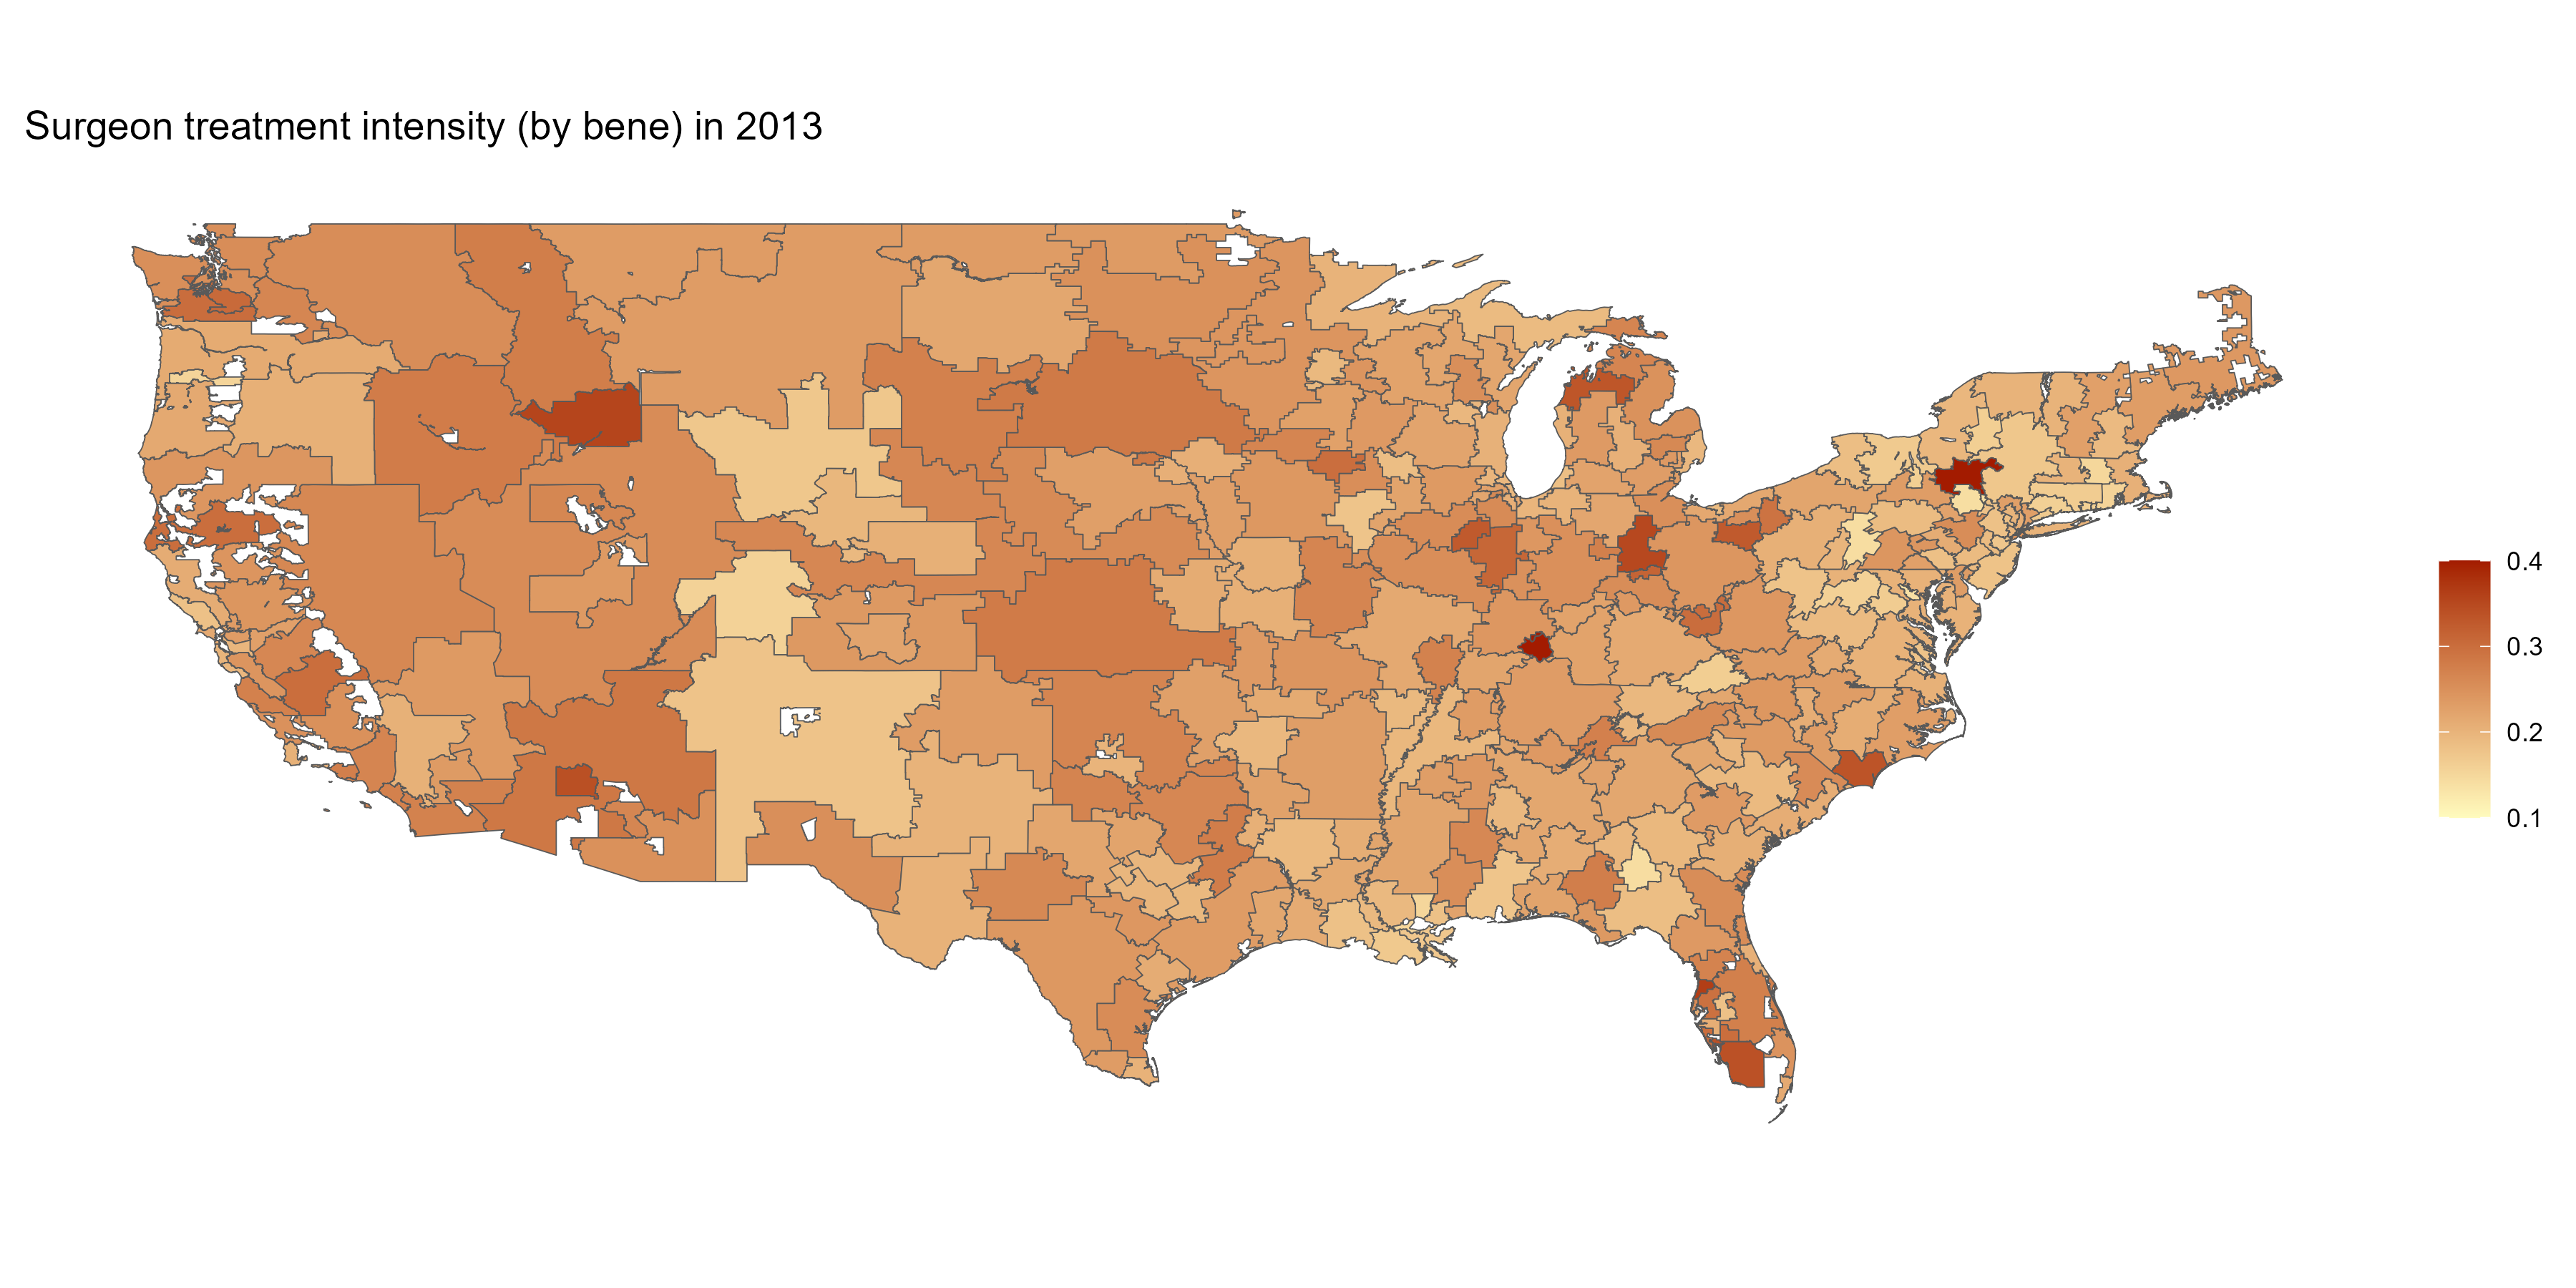
\includegraphics[width=\textwidth]{surg2013.png}
         \label{fig:surg2013}
     \end{subfigure}
     \hfill
     \begin{subfigure}[b]{0.45\textwidth}
         \centering
         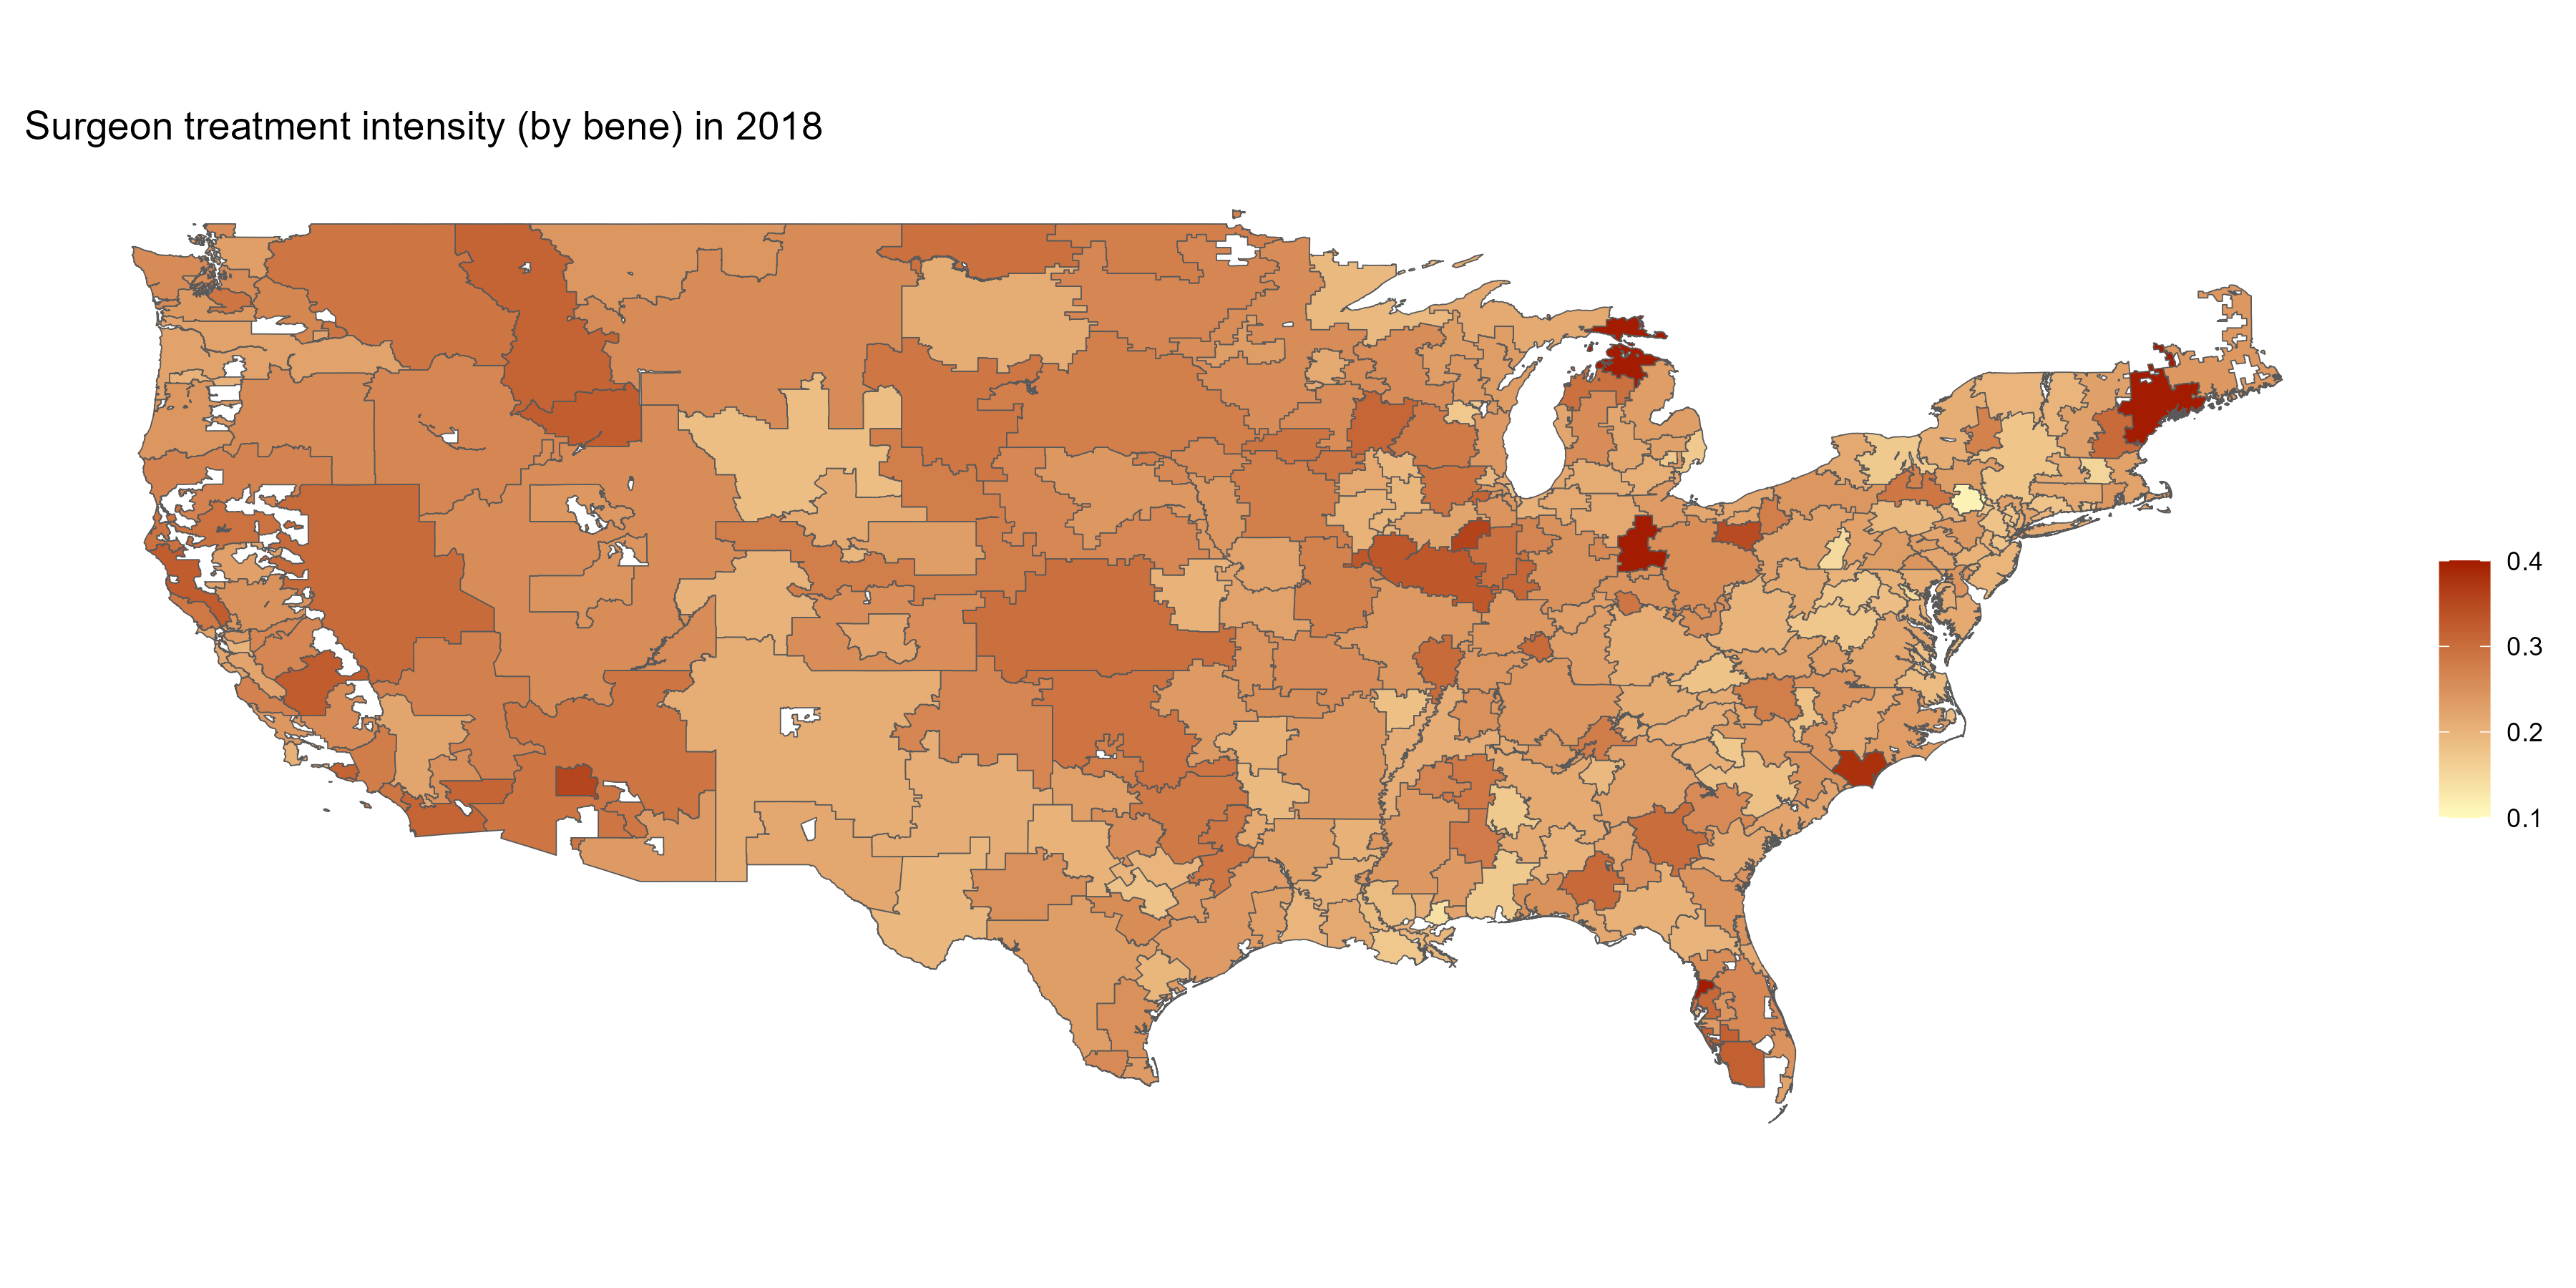
\includegraphics[width=\textwidth]{surg2018.png}
         \label{fig:surg2018}
     \end{subfigure}
    \caption{Treatment intensity by HRR}
    \label{fig:surg-hrr}
\end{figure}

\subsection{Physician Location}
Physician zip codes are identified from Medicare Data on Provider Practice and Specialty (MD-PPAS) for 2013-2018 and from Physician Compare for 2019-2022. Physician practice addresses can also be found in the National Plan and Provider Enumeration System (NPPES) for this time period. However, location in NPPES is only updated when a physician chooses to update it, and this information may be inaccurate or outdated as a result. Addresses from MD-PPAS and Physician Compare are aggregated from Medicare claims, which allows me to determine physician location with greater certainty. From these addresses, I use zip code to assign each physician-year observation to their current practice HRR. 

There are a number of physicians who bill from multiple zip codes. This is not a problem for location reported in MD-PPAS, since it reports the primary zip code of a practitioner based on the number of services performed. The information needed to create a similar primary zip code variable for Physician Compare cannot be linked to each practice location. Within the Physician Compare data, I only consider physicians practicing in one core-based statistical area (CBSA) since these physicians likely have a single, primary practice area. I then assign HRR based on zip code and only keep observations with both a medical school HRR and a single current practice HRR. I define physician movers as those who practice in a HRR different from the HRR where they completed medical school.

\subsection{Other Included Variables}
I also control for physician characteristics and aggregate Medicare patient characteristics for all beneficiaries seen by the physician that year. Physician characteristics include gender, graduation year, and indicators for surgical subspecialty. Aggregate Medicare patient characteristics include average age, proportion female, proportion Black, proportion dual-enrolled in Medicaid, and average hierarchical condition category (HCC) risk score. Dual-enrollment in Medicaid serves as a proxy for the proportion of the physician's patient population that is low-income. HCC risk score is a risk-adjusted estimate of a patient's healthcare costs, and a higher score is indicative of higher expected spending. I use this as a proxy for case-mix, since patients whose cases are more severe may require more surgical treatment. All physician and patient characteristics are from in the PUF, except for graduation year, which is from Physician Compare. I include indicator variables for missing patient characteristics to maintain sample size.

\newcommand*{\tabindent}{ \hspace{3mm}}

\setlength{\LTpost}{0mm}
\LTcapwidth=\textwidth
\begin{ThreePartTable}
\begin{TableNotes}[para, flushleft]
    \textit{Notes.} Missing patient characteristics imputed with unconditional mean among sample to retain sample size.
\end{TableNotes}
\begin{longtable}{lccccc}
    \label{tab:summ} \\
    \caption{Summary statistics} \\
    \toprule
    \multicolumn{1}{l}{Variable} & Mean & Std. Dev & Min & Max & N \\ 
    \midrule\addlinespace[2.5pt]
    \multicolumn{6}{l}{\textbf{Treatment Intensity}} \\ 
    \midrule\addlinespace[2.5pt]
    \tabindent Physician intensity & $0.21$ & $0.45$ & $0$ & $17.977$ & $6,760$ \\ 
    \tabindent Med school HRR intensity & $0.22$ & $0.031$ & $0.122$ & $0.423$ & $6,760$ \\ 
    %\tabindent Med school teaching hospital intensity & - & - & - & - & - \\ 
    \multicolumn{6}{l}{Physician Characteristics} \\ 
    \midrule\addlinespace[2.5pt]
    \tabindent Mover & $0.854$ & $0.354$ & $0$ & $1$ & $6,760$ \\ 
    \tabindent Female & $0.305$ & $0.46$ & $0$ & $1$ & $6,760$ \\ 
    \tabindent Graduation year & $2013.928$ & $1.05$ & $2013$ & $2018$ & $6,760$ \\ 
    \tabindent Cardiac surgeon & $0.003$ & $0.05$ & $0$ & $1$ & $6,760$ \\ 
    \tabindent Colorectal surgeon & $0.002$ & $0.044$ & $0$ & $1$ & $6,760$ \\ 
    \tabindent General surgeon & $0.107$ & $0.309$ & $0$ & $1$ & $6,760$ \\ 
    \tabindent Gynecologic oncologist & $0.001$ & $0.027$ & $0$ & $1$ & $6,760$ \\ 
    \tabindent Hand surgeon & $0.008$ & $0.089$ & $0$ & $1$ & $6,760$ \\ 
    \tabindent Neurosurgeon & $0.011$ & $0.105$ & $0$ & $1$ & $6,760$ \\ 
    \tabindent OBGYN & $0.051$ & $0.22$ & $0$ & $1$ & $6,760$ \\ 
    \tabindent Ophthalmologist & $0.37$ & $0.483$ & $0$ & $1$ & $6,760$ \\ 
    \tabindent Orthopedic surgeon & $0.201$ & $0.401$ & $0$ & $1$ & $6,760$ \\ 
    \tabindent Otolaryngologist (ENT) & $0.114$ & $0.318$ & $0$ & $1$ & $6,760$ \\ 
    \tabindent Plastic surgeon & $0.003$ & $0.058$ & $0$ & $1$ & $6,760$ \\ 
    \tabindent Surgical oncologist & $0.002$ & $0.042$ & $0$ & $1$ & $6,760$ \\ 
    \tabindent Thoracic surgeon & $0.004$ & $0.064$ & $0$ & $1$ & $6,760$ \\ 
    \tabindent Urologist & $0.108$ & $0.31$ & $0$ & $1$ & $6,760$ \\ 
    \tabindent Vascular surgeon & $0.014$ & $0.117$ & $0$ & $1$ & $6,760$ \\ 
    \midrule\addlinespace[2.5pt]
    \multicolumn{6}{l}{Patient Characteristics} \\ 
    \midrule\addlinespace[2.5pt]
    \tabindent Average age & $72.921$ & $3.009$ & $43$ & $84$ & $6,760$ \\ 
    \tabindent Proportion female & $0.568$ & $0.148$ & $0$ & $1$ & $6,760$ \\ 
    \tabindent Proportion Black & $0.142$ & $0.087$ & $0$ & $0.887$ & $6,760$ \\ 
    \tabindent Proportion dual-enrolled & $0.196$ & $0.128$ & $0$ & $1$ & $6,760$ \\ 
    \tabindent Average HCC risk score & $1.445$ & $0.728$ & $0.53$ & $11.413$ & $6,760$ \\ 
    \tabindent Proportion female missing & $0.023$ & $0.15$ & $0$ & $1$ & $6,760$ \\ 
    \tabindent Proportion Black missing & $0.625$ & $0.484$ & $0$ & $1$ & $6,760$ \\ 
    \tabindent Proportion dual-enrolled missing & $0.155$ & $0.362$ & $0$ & $1$ & $6,760$ \\ 
    \bottomrule
    \insertTableNotes
\end{longtable}
\end{ThreePartTable}


\subsection{Sample Restrictions}
All treatment intensity measures are based on surgeries performed on Medicare beneficiaries with part B fee-for-service coverage. These patients are older than the general population and could experience more harm from surgery; thus, treatment intensity may be lower for this patient group compared to a more general one. Further, fee-for-service beneficiaries are likely less healthy than those in Medicare Advantage due to selection. Due to age and other risk factors, it is probable that physicians are less likely to deviate from treatment norms either from their training or from their current workplace. That is, the Medicare population is less healthy compared to the general population, and physicians may tend to choose treatment decisions that are more ``by the book" and more impacted by medical school training. As a result, the magnitude of any result found here can be thought of as an upper bound for the general patient population.


\section{Empirical Estimation}
% Last updated: 2025/04/22

% Main specification
Upon graduating from residency and fellowship, physicians migrate out of necessity. There will be those who begin practice in a different market than the one they trained in, who I call ``movers", and those who stay in the market they trained in, who I call ``stayers". The core of my identification strategy is to compare physician movers to stayers while controlling for influences from their current market. This utilizes the fact that movers who train in a different market are exposed to a different intensity level in medical school compared to stayers. The primary specification is 
    \begin{align} \label{eq:main}
        intensity_{it} 
        &= \beta (mover_i \times \textit{med school HRR intensity}_{it_g}) \nonumber\\
        &\quad + \psi \textit{med school HRR intensity}_{it_g} + \theta X_{i} + \eta M_{it} \nonumber\\
        &\quad + \gamma_i + \tau_t + \epsilon_{it},
    \end{align}
where $intensity_{it}$ is physician $i$'s treatment intensity in year $t$, $mover_i$ is an indicator that physician $i$'s current practice HRR is different from their medical school HRR, and $\textit{med school HRR intensity}_{it_g}$ is the average treatment intensity in physician $i$'s medical school HRR in year of graduation $t_g$. The vector $X_i$ contains physician characteristics, and the vector $M_{it}$ contains variables that reflect the physician's Medicare patient population, as described above. All models include current HRR fixed effects $\gamma_i$ and year fixed effects $\tau_t$. Standard errors are clustered at the current HRR level due to spacial correlation. 

% Semi-parametric specification
I estimate equation \ref{eq:main} using OLS, which assumes that the effect of medical school intensity on a physician's current intensity is linear. However, one can easily imagine that more extreme medical school intensities will have a greater impact. For this reason, I also semi-parametrically estimate equations of the following form: 
    \begin{align} \label{eq:spline}
        intensity_{it} 
        &= f(\textit{med school HRR intensity}_{it_g}) \times mover_i \nonumber\\
        &\quad + \theta X_{i} + \eta M_{it} + \gamma_i + \tau_t + \epsilon_{it},
    \end{align}
where $f(\cdot)$ is estimated using a cubic spline. 

These two specifications capture the effect of the level of medical school intensity. However, they fail to acknowledge that some movers now practice in more intense HRRs compared to their medical school, while others practice in less intense HRRs compared to their medical school. To account for this fact, I additionally estimate equations using the difference between current HRR intensity and medical school intensity. 
    \begin{align} \label{eq:delta}
        intensity_{it} 
        &= \beta (mover_i \times \textit{change in intensity}_{it}) \nonumber\\
        &\quad + \psi \textit{med school HRR intensity}_{it_g} + \theta X_{i} + \eta M_{it} \nonumber\\
        &\quad + \gamma_i + \tau_t + \epsilon_{it},
    \end{align}
where $\textit{change in intensity}_{it}$ is defined as the difference between the leave-one-out mean intensity of physician $i$'s current HRR in year $t$, excluding physician $i$, and the average treatment intensity in physician $i$'s medical school HRR in their year of graduation. 

% Endogeneity concerns
There are two potential sources for endogeneity: reverse causality and omitted variable bias. It is likely that average HRR intensities are changing over time due to physician movement. Since my medical school intensity measures are calculated at the time the physician graduates from medical school, reverse causality is not an issue. Omitted variable bias is a greater concern here. It is possible that medical schools are investing in new technology, and this improvement in technology is what is actually responsible for both changes in market-level treatment intensity as well as the intensity of graduating physicians. It may be possible to account for this using AHA survey data and requires further analysis. 


\section{Results}
% Last updated: 2025/04/22

\subsection{Descriptive comparison}
Figure \ref{fig:scatter} shows a simple scatterplot comparison between a surgeon's current treatment intensity and their medical school HRR intensity. As evidenced by the graph, there seems to be little difference between the mover and stayer groups. This descriptive result will be quantified with later estimates. Interestingly, about 67\% of surgeons in my sample practice less intensely than the average intensity they were exposed to in medical school. This proportion is similar among movers and stayers, though slightly higher in the stayer group (70\%). This below-average intensity is likely due to the fact that newer surgeons with less experience may be more selective about when to operate due to lack of experience. 

\begin{figure}
     \centering
     \begin{subfigure}[b]{0.45\textwidth}
         \centering
         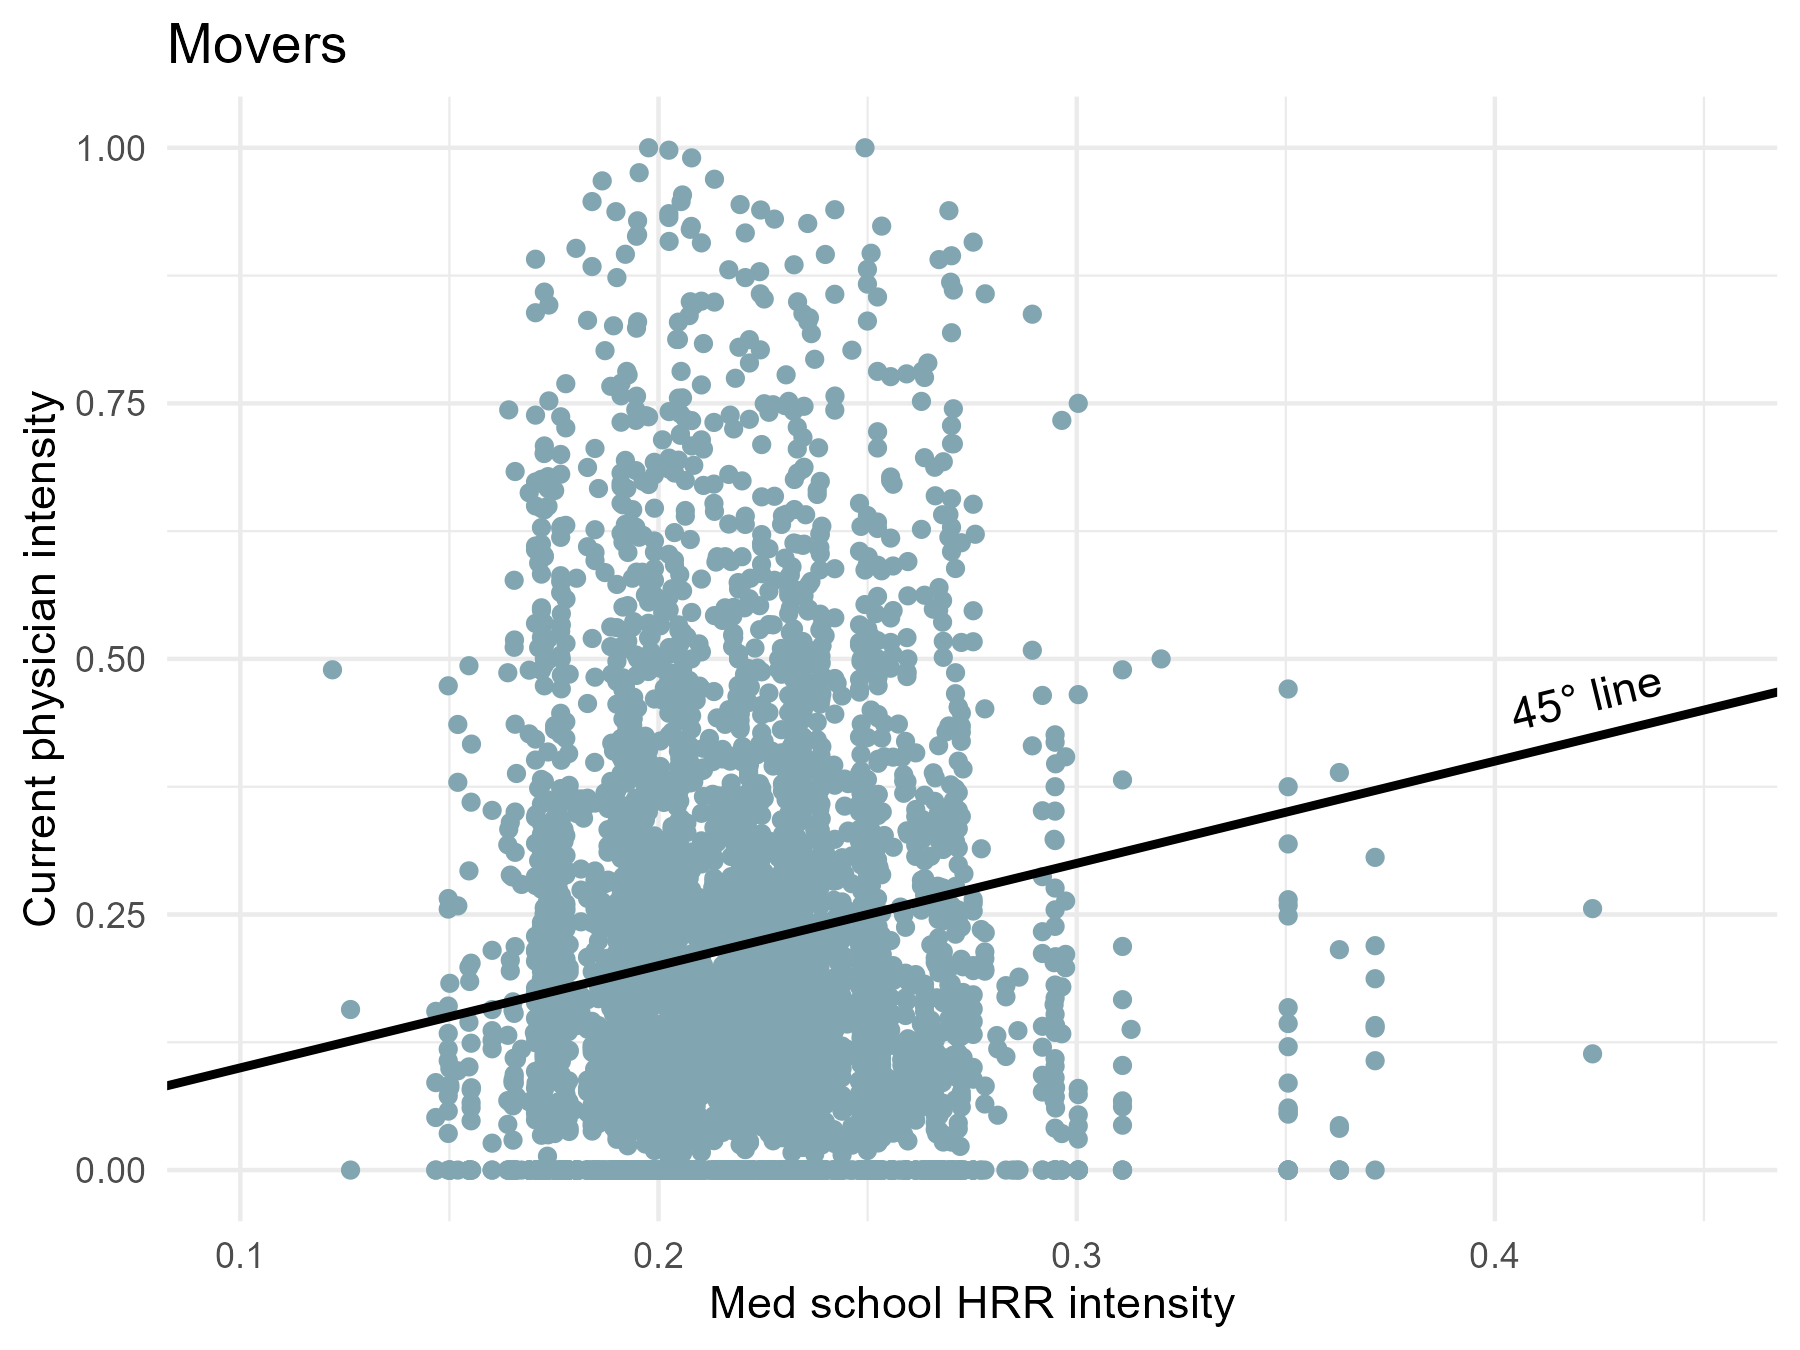
\includegraphics[width=\textwidth]{intensity_corr_movers.png}
         \label{fig:scatter-movers}
     \end{subfigure}
     \hfill
     \begin{subfigure}[b]{0.45\textwidth}
         \centering
         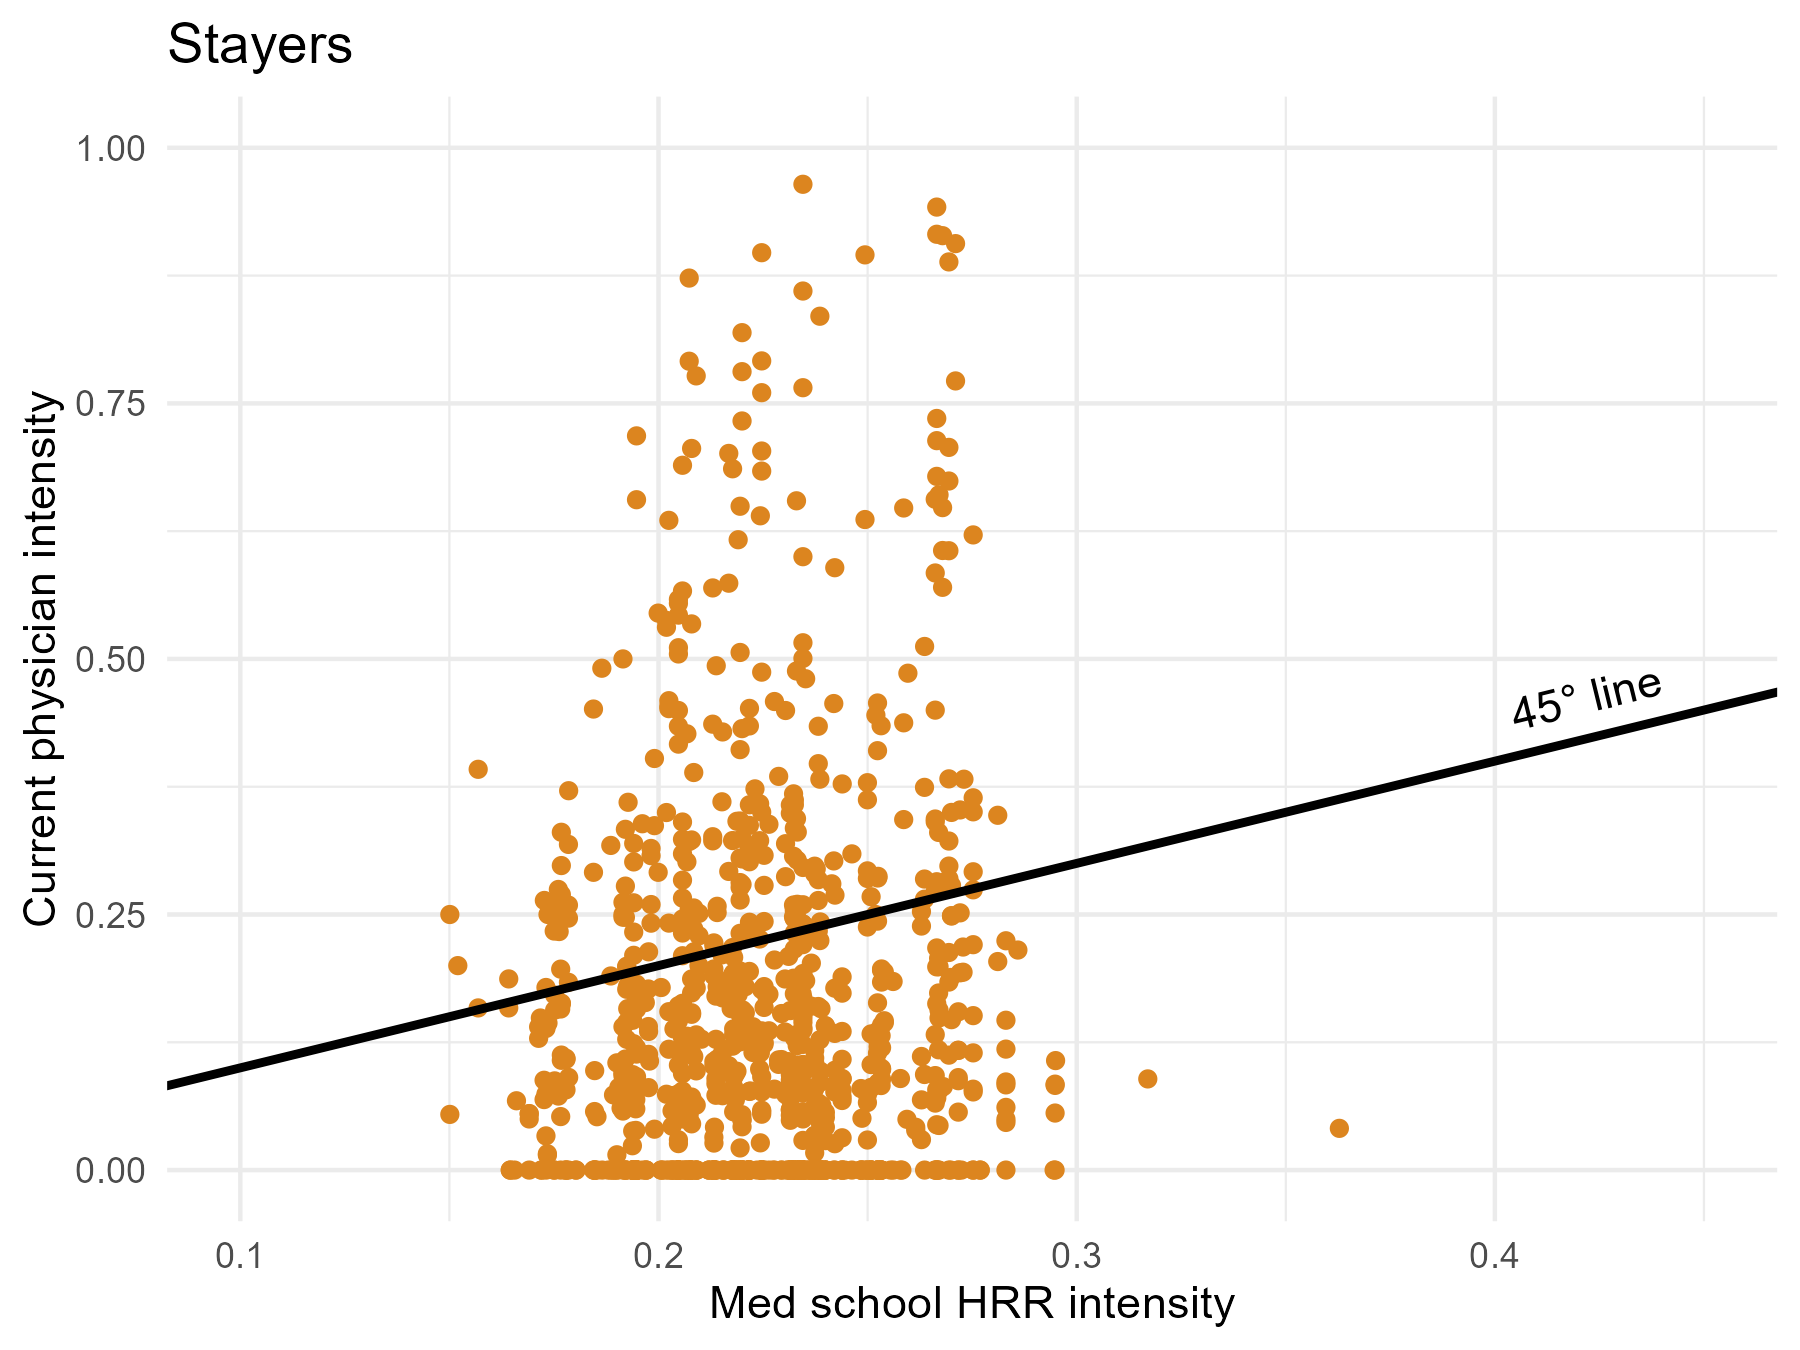
\includegraphics[width=\textwidth]{intensity_corr_stayers.png}
         \label{fig:scatter-stayers}
     \end{subfigure}
    \caption{Correlation between med school HRR intensity and current intensity}
    \label{fig:scatter}
\end{figure}

\subsection{Effect of level of medical school intensity}
In Table \ref{tab:res-main-short}, I present the main estimates of equation \ref{eq:main}. I estimate the equation in the full sample of all surgeons, as well as two subgroups consisting of only general surgeons and only specialist surgeons. I consider a specialist surgeon to be any surgeon whose specialty is not general surgery. General surgeons undergo residency training that is often the basis for other surgical subspecialties. I expect to see a larger impact of medical school within generalists, since they tend to undergo less GME compared to surgical specialists. 

\setlength{\LTpost}{0mm}
\LTcapwidth=\textwidth
\begin{ThreePartTable}
\begin{TableNotes}[para, flushleft]
    \textit{Notes.} Clustered standard errors are based on the physician's current HRR Model 1 includes indicators for all surgical subspecialties, and model 3 includes indicators for surgical subspecialties other than vascular surgery. All models include physician gender, patient characteristics, and indicators for missing patient characteristics, as shown in Table \ref{tab:summ}. All models also include current HRR fixed effects and year fixed effects. $* p < 0.10, ** p < 0.05, *** p < 0.01$.
\end{TableNotes}
\begin{longtable}{lccc}
    %\centering
    \label{tab:res-main-short} \\
    \caption{Effect of medical school intensity on physician own intensity} \\
    %\begin{tabular}{lccc}
        \toprule
         & (1) & (2) & (3) \\
         & All surgeons & Generalists & Specialists \\
        \midrule
        Mover $\times$ med school HRR intensity & -0.017 & 0.134 & -0.018 \\ 
         & (0.106) & (0.093) & (0.117) \\ 
        Med school HRR intensity & -0.223 & -0.203 & -0.237 \\ 
         & (0.278) & (0.222) & (0.313) \\ 
        \midrule
        Observations & 6760 & 723 & 6037 \\ 
        $R^2$ & 0.233 & 0.725 & 0.231 \\ 
        Mean physician intensity & 0.210 & 0.139 & 0.219 \\ 
        \bottomrule
        \insertTableNotes
    %\end{tabular}
\end{longtable}
\end{ThreePartTable}


The effect of medical school HRR intensity is statistically insignificant across the board. Examining the magnitude of effect for the full sample reveals that medical school seems to have no meaningful effect on how a physician practices now. A 1 percentage point increase in medical school HRR intensity decreases a surgeon's current treatment intensity by about 0.017 percentage points compared to their peers in the same destination HRR. This corresponds to about a 0.08\% decrease in treatment intensity. Although this is not a tight null, the 95\% confidence interval suggests that the effect of one percentage point increase in medical school HRR intensity ranges between a 1\% decrease and a 1\% increase in current physician intensity. The entire range is not economically meaningful. The effect estimated within the specialist subsample is similarly both statistically and economically insignificant. 

The magnitude of the effect within the generalist subsample is larger, as expected, but still statistically insignificant. A positive effect here indicates that general surgeons who attended medical school in more intense areas practice more intensely compared to their current peers. The effect size is still small, however. A 1 percentage point increase in medical school HRR intensity increases a general surgeon's current practice intensity by 0.134 percentage points, which corresponds to about a 1\% increase in intensity. The 95\% confidence interval suggests that the effect is ranges between a -0.35\% decrease and a 2.3\% increase.

Estimates of the semi-parametric specification in equation \ref{eq:spline} reveal that the effect of medical school intensity is not much different at the tails, although estimates are fairly noisy. In Figures \ref{fig:spline}, I present predicted physician intensity using only the cubic spline term. The magnitudes of predicted physician intensity when predicting using the mean of all other covariates is similar, but much noisier. The unadjusted effect of medical school intensity is small, and medical school intensity does not have a differential effect between movers and stayers. 
\begin{figure}
     \centering
     \begin{subfigure}[b]{0.3\textwidth}
         \centering
         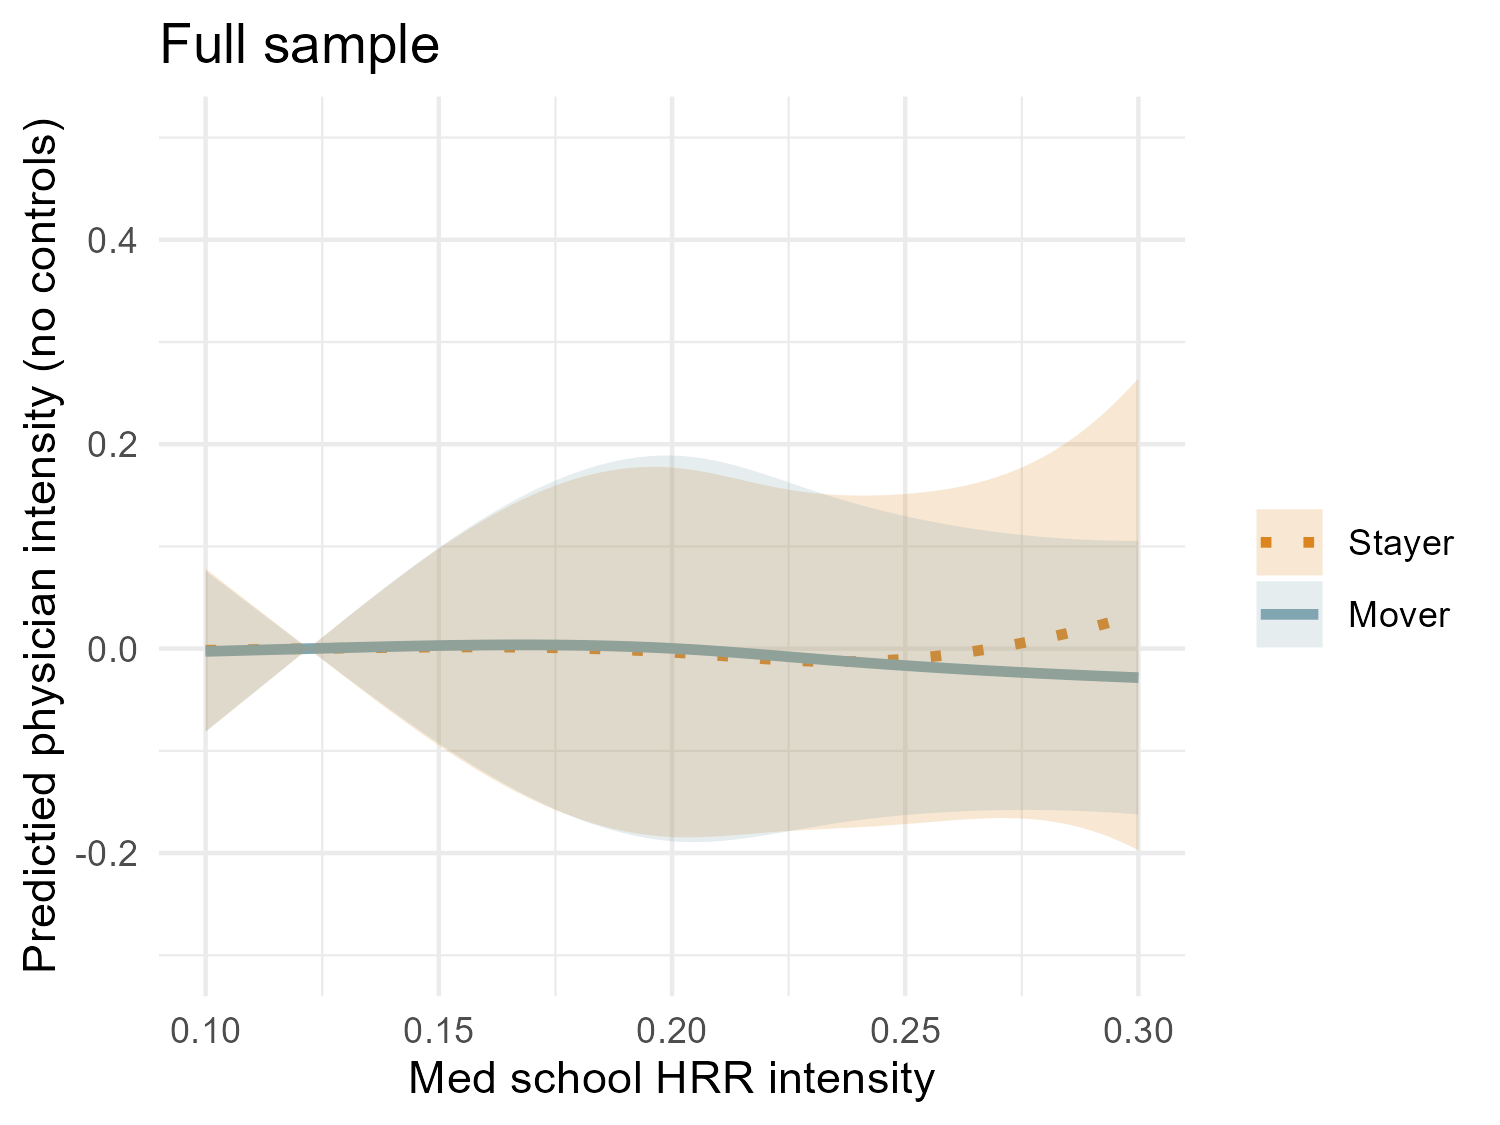
\includegraphics[width=\textwidth]{spline-full.png}
         \label{fig:spline-full}
     \end{subfigure}
     \hfill
     \begin{subfigure}[b]{0.3\textwidth}
         \centering
         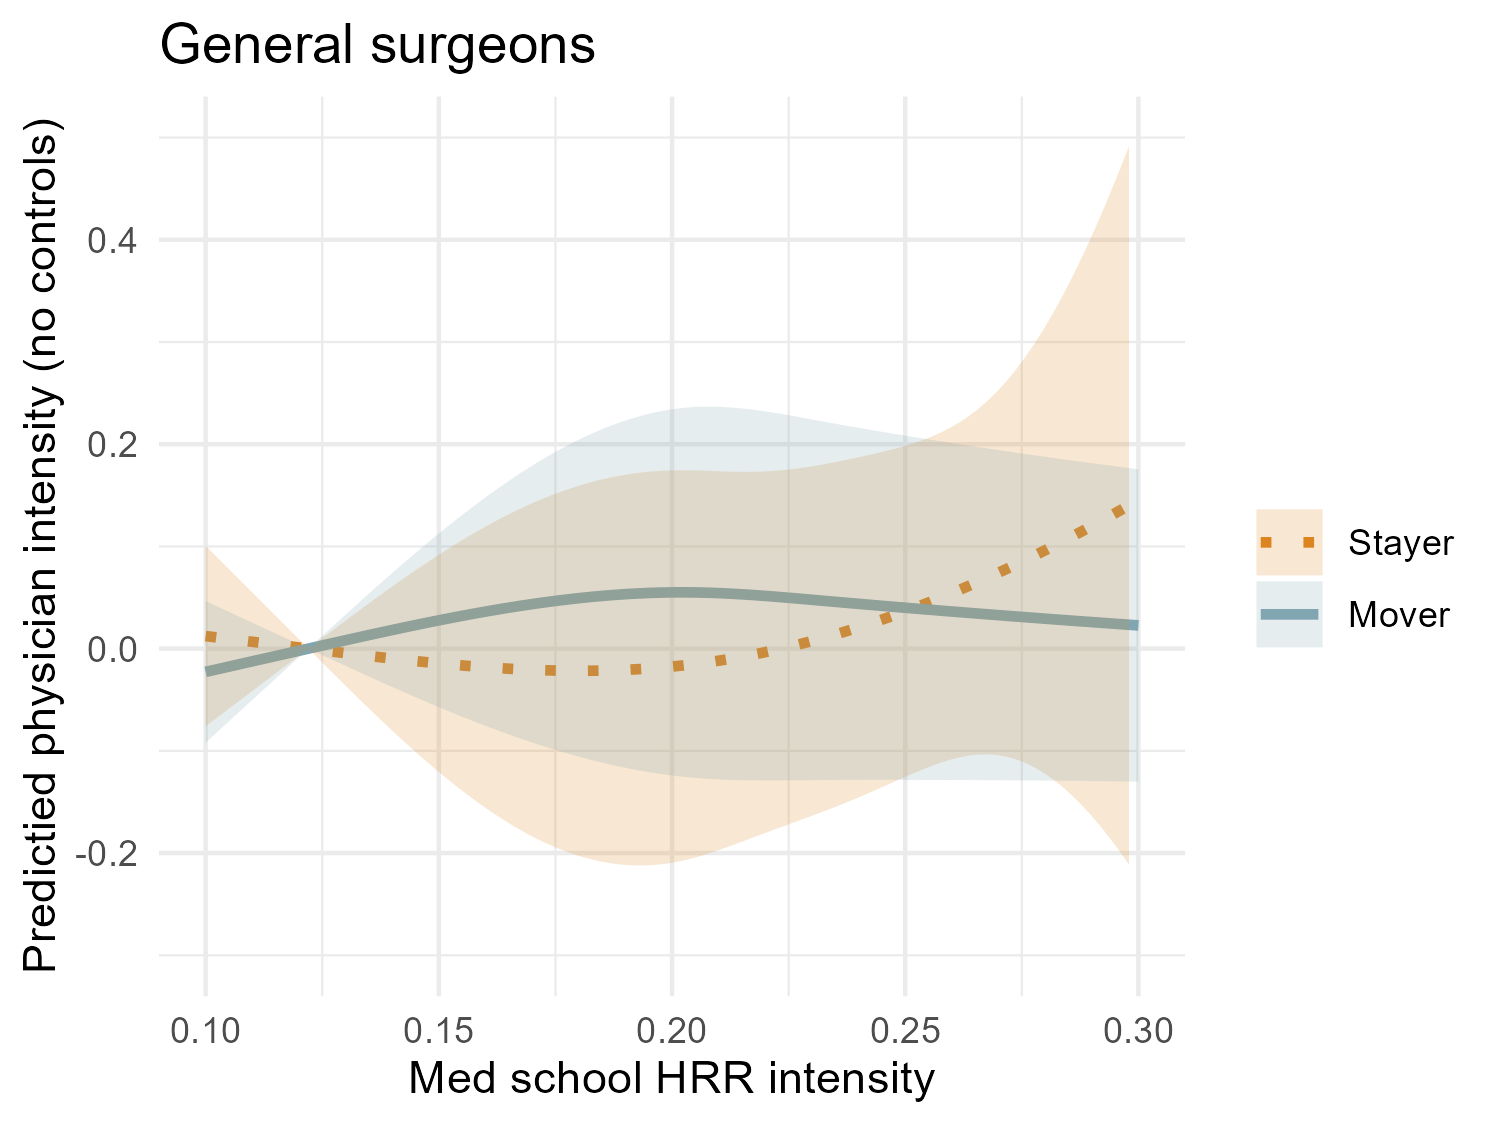
\includegraphics[width=\textwidth]{spline-general.png}
         \label{fig:spline-general}
     \end{subfigure}
     \hfill
     \begin{subfigure}[b]{0.3\textwidth}
         \centering
         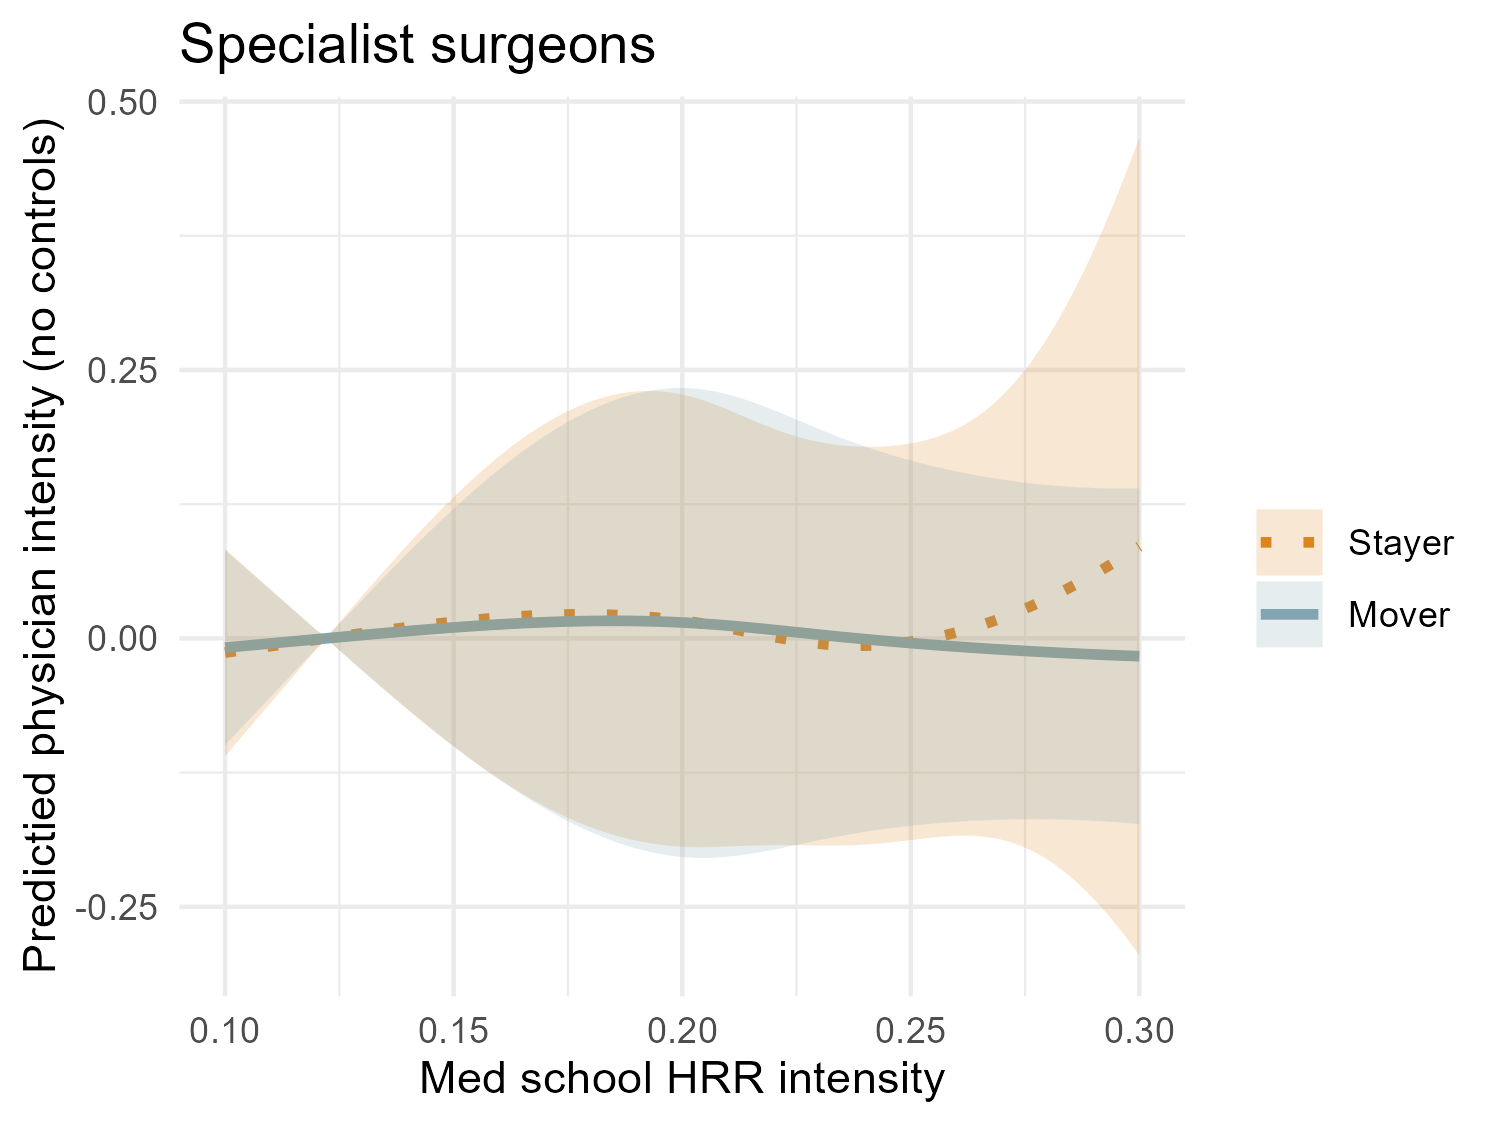
\includegraphics[width=\textwidth]{spline-specialist.png}
         \label{fig:spline-specialist}
     \end{subfigure}
    \caption{Predicted physician intensity without controls}
    \label{fig:spline}
\end{figure}

\subsection{Effect of difference in intensity}
Results from specifications utilizing the change in intensity from medical school HRR to destination HRR tell a slightly different story compared to examining the level of medical school intensity alone. The raw level of medical school intensity does not seem to have an effect, which may be confounded by some surgeons moving to more intense areas, while other surgeons move to less intense areas. Estimates of equation \ref{eq:delta} allows for greater comparison using the differences between the intensity in the training market compared to the practice market. 

Estimated effects are presented in Table \ref{tab:res-delta-short}. Results in the full sample and specialist sample are statistically significant at the 0.10 level, but not at the 0.05 level. The negative sign here indicates that an increase in the difference between a surgeon's current practice HRR and their medical school decreases their current treatment intensity relative to their peers in the same current HRR. That is, the more intense a surgeon's current practice HRR is compared to their medical school HRR, the more they tend to practice less intensely compared to their peers. Specifically, the increasing the difference by 1 percentage point decreases a surgeon's current practice intensity by 2.5 percentage points. This corresponds to a 12\% decrease. The 95\% confidence interval suggests the effect is between a 26\% decrease and a 2\% increase. It's possible that surgeons who train in less intense areas adjust their treatment intensity to accommodate norms in their current practice market, but only to the extent of the support of their medical school HRR intensity distribution. Further work, perhaps with more granular data, is needed to determine how the distribution of the medical school HRR impacts current practice intensity in a way beyond just the mean. 

\setlength{\LTpost}{0mm}
\LTcapwidth=\textwidth
\begin{ThreePartTable}
\begin{TableNotes}[para, flushleft]
    \textit{Notes.} Clustered standard errors are based on the physician's current HRR Model 1 includes indicators for all surgical subspecialties, and model 3 includes indicators for surgical subspecialties other than vascular surgery. All models include physician gender, patient characteristics, and indicators for missing patient characteristics, as shown in Table \ref{tab:summ}. All models also include current HRR fixed effects and year fixed effects. $* p < 0.10, ** p < 0.05, *** p < 0.01$.
\end{TableNotes}
\begin{longtable}{lccc}
    %\centering
    \label{tab:res-delta-short} \\
    \caption{Effect of change in intensity on physician own intensity} \\
    %\begin{tabular}{lccc}
        \toprule
         & (1) & (2) & (3) \\
         & All surgeons & Generalists & Specialists \\
        \midrule
        Mover $\times$ change in intensity & -2.544* & -0.412 & -2.919* \\ 
         & (1.503) & (0.323) & (1.701) \\ 
        Med school HRR intensity & -2.783* & -0.505 & -3.171* \\ 
         & (1.664) & (0.389) & (1.881) \\ 
        \midrule
        Observations & 6760 & 723 & 6037 \\ 
        $R^2$ & 0.241 & 0.723 & 0.241 \\ 
        Mean physician intensity & 0.210 & 0.139 & 0.219 \\
        \bottomrule
        \insertTableNotes
    %\end{tabular}
\end{longtable}
\end{ThreePartTable}


These findings suggest that medical school intensity does not have a statistically or economically significant effect on a physician's current practice. Overall, this provides support for the story where medical school provides a foundational knowledge base, but practical knowledge about patient types and when to operate is developed and refined in residency and fellowship, contrary to popular belief. It's possible that medical knowledge is taught differently in medical schools, but the information that a surgeon retains from medical school about treatment intensity seems to be somewhat standardized. 

\section{Conclusions}
% Last reviseed: 2025/04/24
 
Surgeons have considerable discretion in the decision to operate. Previous literature has established that factors in a physician's current practice environment continues to evolve their practice intensity, but the factors that determine their initial baseline for what the standard of care is remains largely unexplored. I use a new measure of the influence of treatment intensity around a physician's medical school alongside a physician mover design in order to determine the effect of medical school on a physician's current intensity.

I show that medical school does not have a statistically or economically significant effect on a surgeon's current practice. Results here provide support for the story that key foundational knowledge is built in medical school, while practical knowledge is built in later stages of training. Future work should explore the role of residency in order to determine the the most important part of the training pipeline, potentially allowing policymakers to target cost-saving initiatives to nip high healthcare expenditures in the bud. 

\clearpage

%%%%%%%%%%%%%%%%%%%%%%%%%%%%%%%%%%%%%%%%%%%%%%%%%
\begin{singlespace}
\bibliographystyle{aer}
\bibliography{BibTeX_Library}
\end{singlespace}
%%%%%%%%%%%%%%%%%%%%%%%%%%%%%%%%%%%%%%%%%%%%%%%%%

\end{document}
